\newpage
\section{Техническое задание}
\subsection{Основание для разработки}

Основанием для разработки является задание на выпускную квалификационную работу бакалавра ``Разработка web-сайта ``Русатом –Аддитивные технологии'' на платформе 1С-Битрикс''.

\subsection{Цель и назначение разработки}

Основной задачей выпускной квалификационной работы является разработка и внедрение web-сайта для продвижения компании ООО «Русатом – Аддитивные технологии».

Посредством внедрения web-сайта планируется устранить существующие недостатки в компании. Исходя из этого, основную цель предлагается рассмотреть в разрезе двух групп подцелей.

Задачами данной разработки являются:
\begin{itemize}
\item создание информационных разделов сайта;
\item    реализация формы для обратной связи;
\item реализация калькулятора расчета стоимости изготовления деталей;
\item реализация формы заявки на изготовление деталей;
\item создание удобного поиска по сайту.
\end{itemize}

\subsection{Требования пользователя к интерфейсу web-сайта}

Сайт должен включать в себя:
\begin{itemize}
    \item навигацию по разделам;
    \item авторизацию;
    \item доступы для администратора, редактора, исполнителя по заявкам с форм.
\end{itemize}

Композиция шаблона сайта представлена на рисунке ~\ref{templ:image}.
\begin{figure}[h]
\center{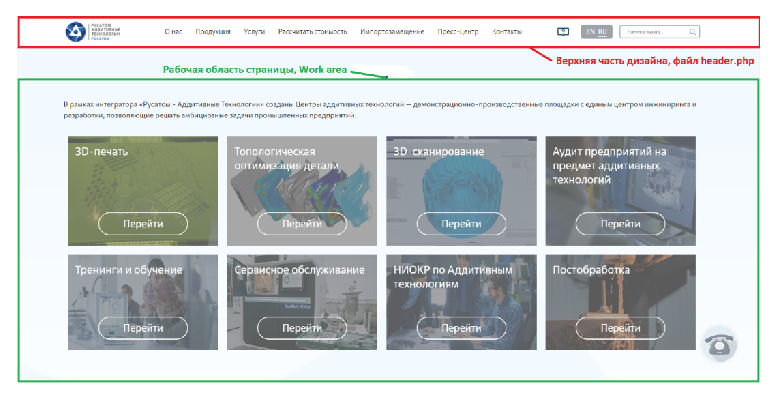
\includegraphics[width=1\linewidth]{templ}}
\caption{Композиция шаблона сайта}
\label{templ:image}
\end{figure}
